%========================================================================================
% TU Dortmund, Informatik Lehrstuhl VII
%========================================================================================

\chapter{Graphbasierte Modellierung des Höchstspannungsnetzes}
\label{Kapitel 2}
%

\section{Höchstspannungsnetz}
\label{Höchstspannungsnetz}
%
\begin{figure}[t]
	\centering
	{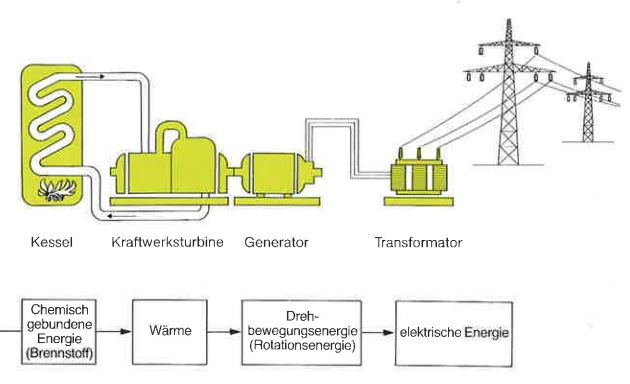
\includegraphics[scale=0.9]{bilder/pds}\label{fig_pds}
	}\\
	\caption[Prinzip der Stromerzeugung]{Prinzip der Stromerzeugung[1]}
	\label{fig_pds}
\end{figure}

\begin{figure}[t]
	\centering
	\subfigure[Niederspannungsleitungen]
	{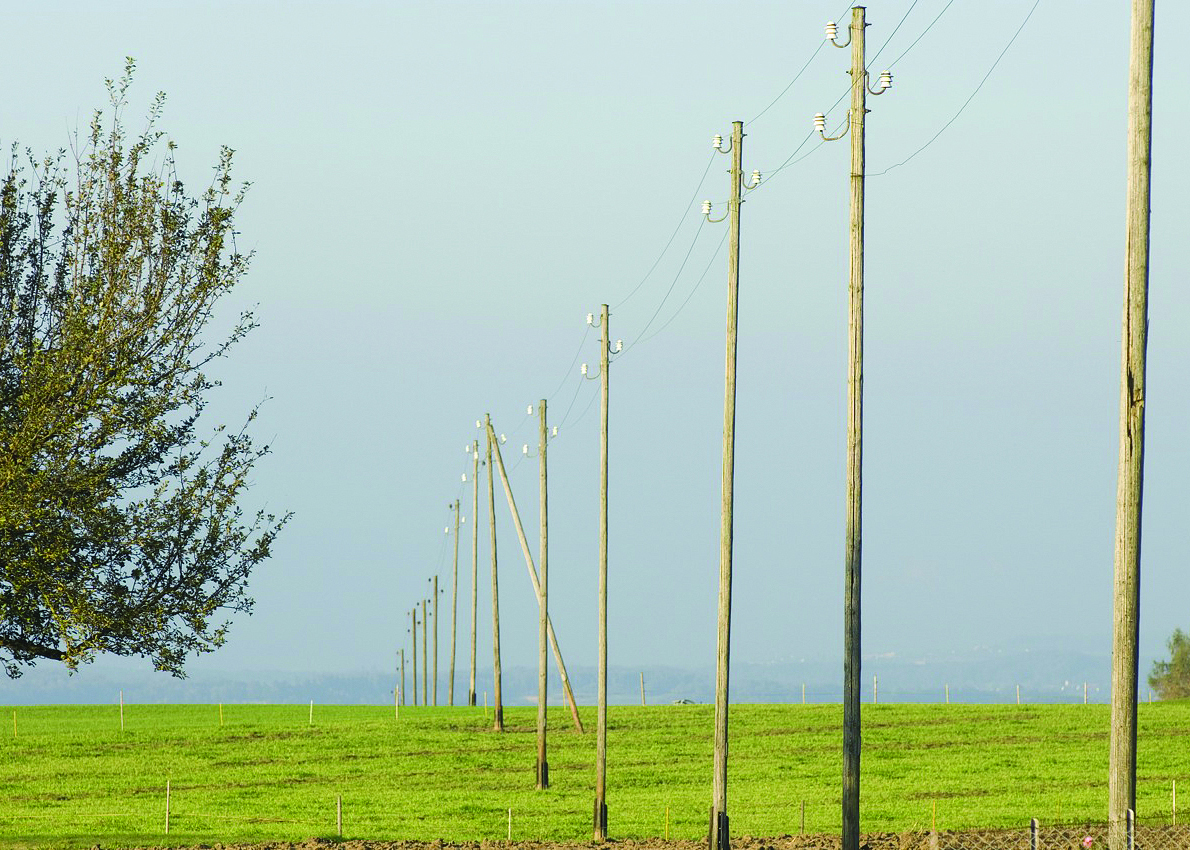
\includegraphics[scale=0.15]{bilder/nieder}\label{fig_nieder}
	}
	\hspace{1.0cm}%
	\subfigure[Mittelspannungsmast]
	{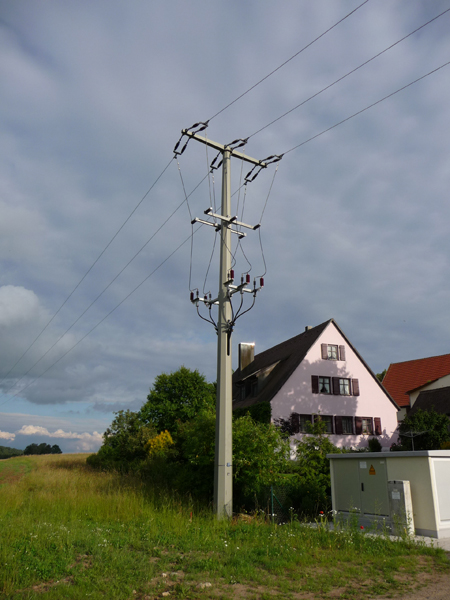
\includegraphics[scale=0.25]{bilder/mittelspannungsleiter}\label{fig_mittelspannungsleiter}
	}
	\hspace{1.0cm}%
	\subfigure[Hochspannungsleitungen]
	{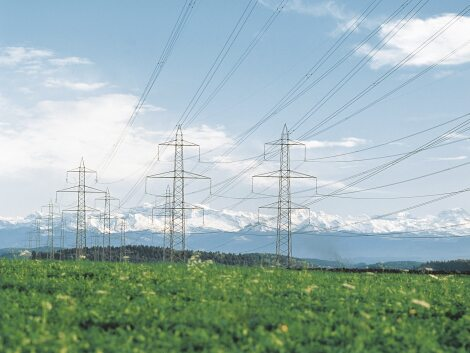
\includegraphics[scale=0.3]{bilder/hochspannungsleitungen}\label{fig_hochspannungsleitungen}
	}
	\hspace{1.0cm}%
	\subfigure[modernisierter Höchstspannungsmast]
	{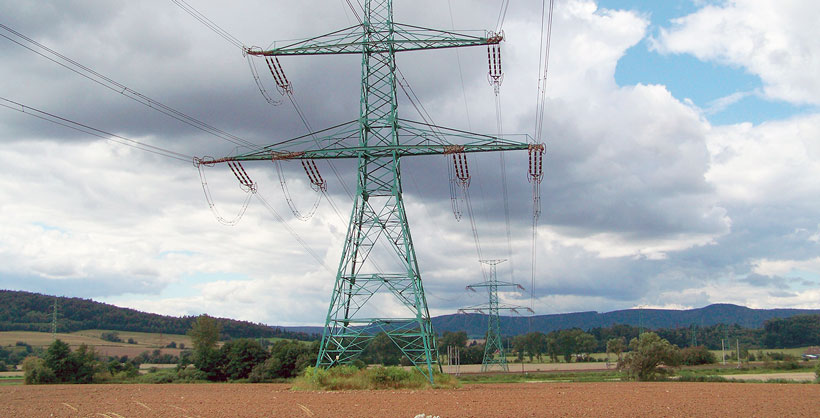
\includegraphics[scale=0.2]{bilder/Reptcheque_HT}\label{fig_Reptcheque_HT}
	}
	\\
	\caption[Die vier verschiedenen Leitungstypen]{Die vier verschiedenen Leitungstypen}
	\label{fig_testbild2}
\end{figure}





\begin{figure}[t]
	\centering
	{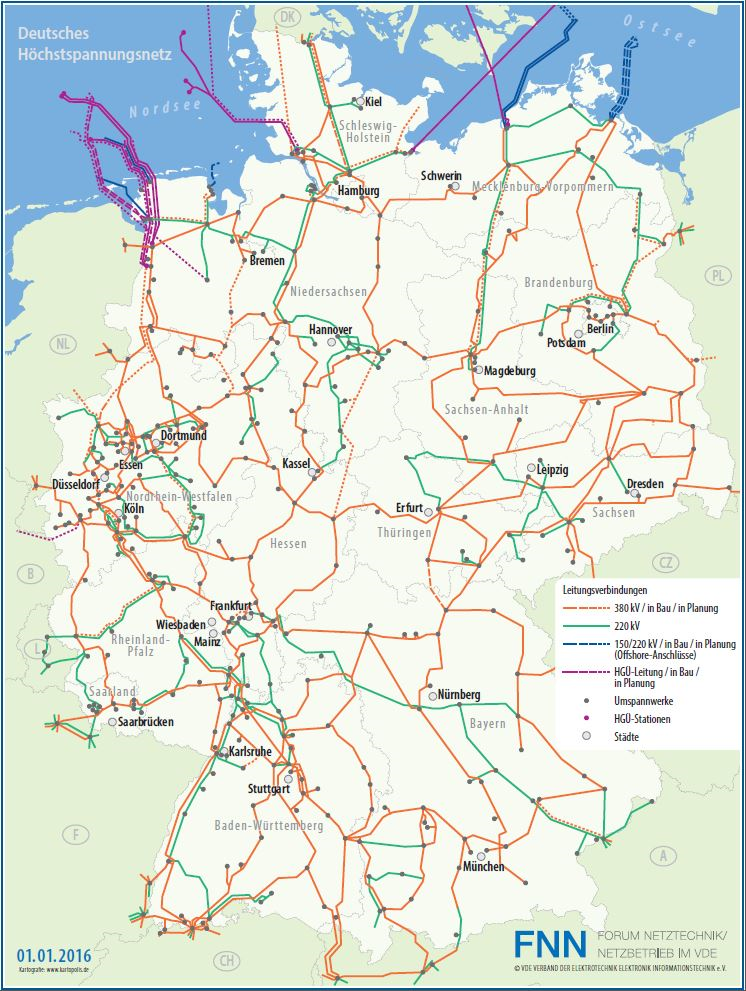
\includegraphics[scale=0.5]{bilder/hochstspannungsnetz}\label{fig_hochstspannungsnetz}
	}\\
	\caption[Karte des deutschen Höchstspannungsnetzes]{Karte des deutschen Höchstspannungsnetzes[1]}
	\label{fig_hochstspannungsnetz2}
\end{figure}
\begin{figure}[t]
	\centering
	{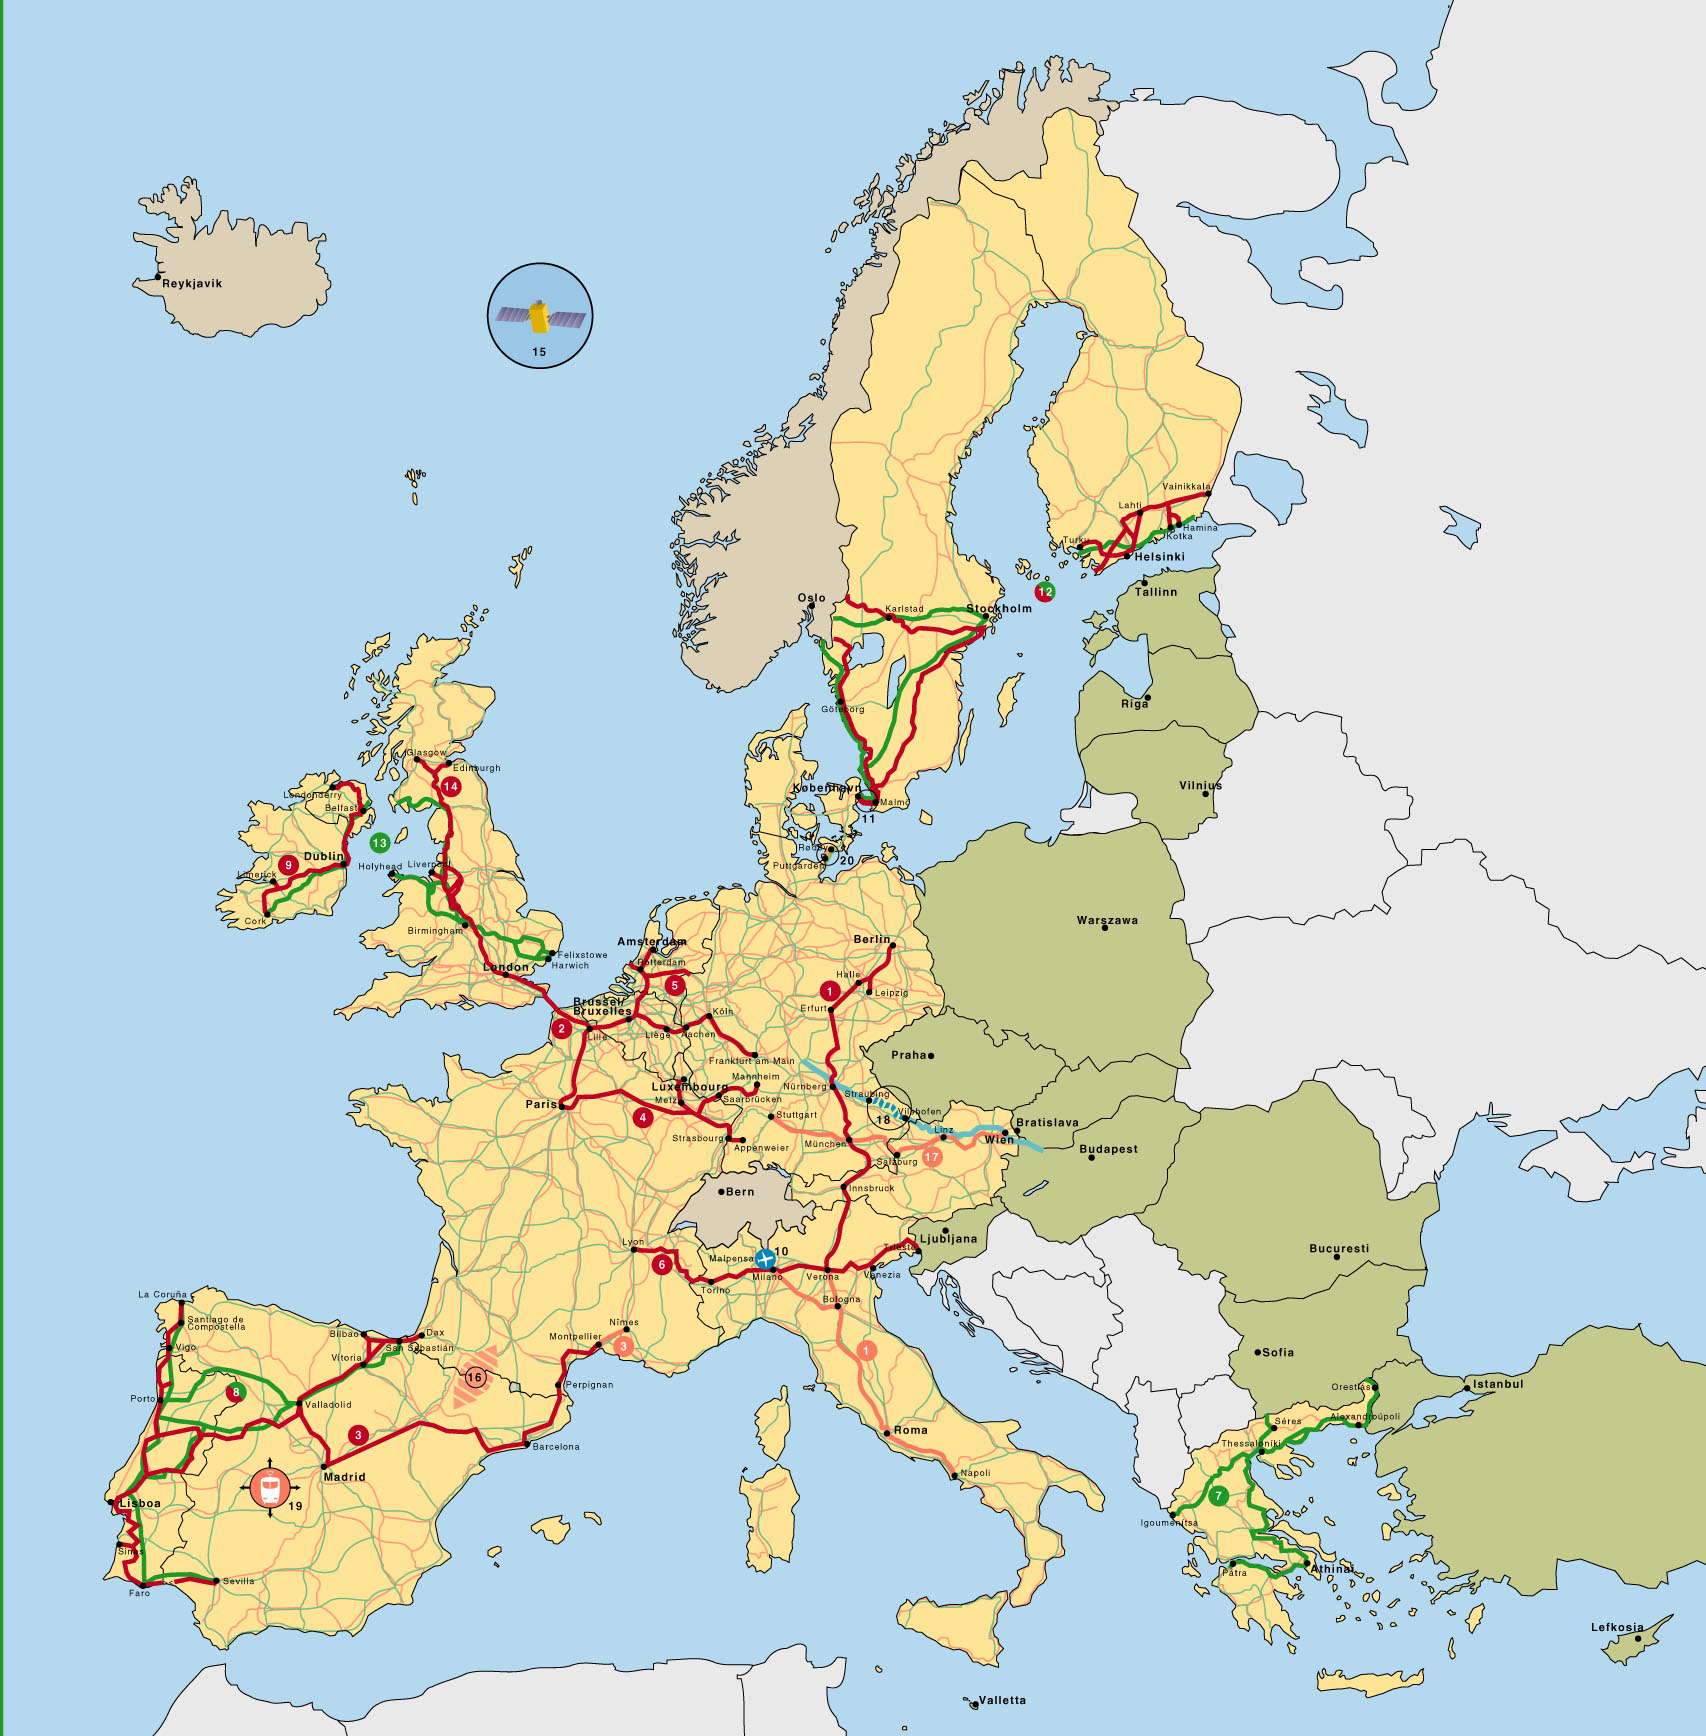
\includegraphics[scale=0.9]{bilder/europastromnetz}\label{fig_europastromnetz}
	}\\
	\caption[Karte des europäischen Verbundnetzes]{Karte des europäischen Verbundnetzes[1]}
	\label{fig_europastromnetz}
\end{figure}

\begin{figure}[t]
	\centering
	{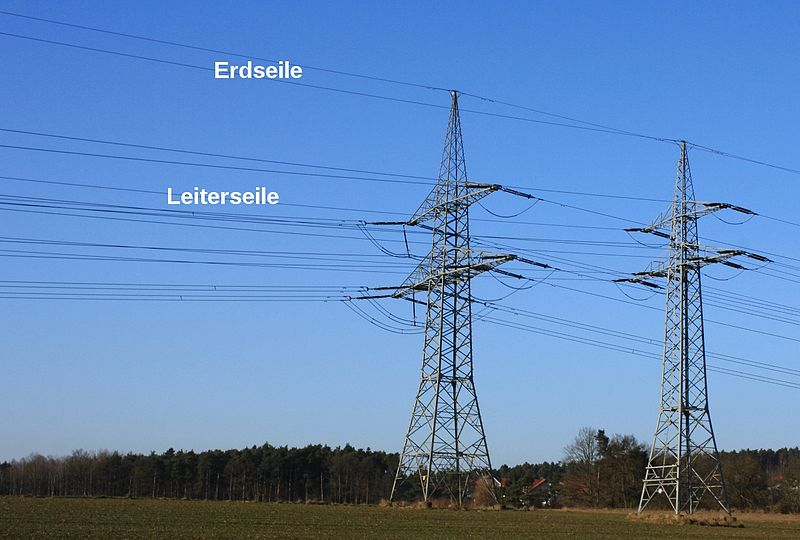
\includegraphics[scale=0.5]{bilder/erdseil}\label{fig_erdseil}
	}\\
	\caption[Freileitungsmast mit Leitern und Erdseil]{Freileitungsmast mit Leitern und Erdseil[1]}
	\label{fig_erdseil}
\end{figure}
Die vorliegenden Ausführungen orientieren sich am Lehrerfachheft "Übertragung und Verteilung der elektrischen Energie".
Um elektrische Energie über große Distanzen zu transportieren werden Höchstspannungsnetze benutzt. Von einem Kraftwerk ausgehend wird versucht möglichst viele Haushalte, Industrie- und Gewerbebetriebe zu erreichen. Davon ausgehend wird auch der Standort der meisten Kraftwerke bestimmt. Einige Kraftwerke lassen sich nur an bestimmten Standorten errichten, zum Beispiel ein Wasserkraftwerk muss an einem Fluss oder Staudamm errichtet werden. So ist es oft nicht möglich genug Verbraucher zu erreichen, sodass es Mittel bedarf den elektrischen Strom auch über weite Strecken hinweg zu transportieren.

Die Generatoren der modernen Kraftwerke erzeugen eine Spannung von $10500 V$, $21000V$ oder $27000V$[1]. Die Höhe dieser Spannung ist bestimmt durch die Größe bzw. die Leistungsfähigkeit des Kraftwerks und somit von der Nennleistung des Generators.

Da der überwiegende Teil der elektrischen Energie in Wärmekraftwerken erzeugt wird und diese mit einer Generatorleistung von $600$ bis $1300MW$, bedeutet dies, dass Ströme zwischen $15000A$ und $30000A$ abgegeben werden müssen. Das ist jedoch weder aus technischen noch wirtschaftlichen Gründen für einen Transport über lange Distanzen lohnenswert, da es entweder sehr großen Leiterquerschnitte oder sehr große Stromverluste zur Folge hätte.

Es kann die gleiche Leistung $P$ auch mit weniger Strom $I$ und einer erhöhten Spannung $U$ erreicht werden, denn die Beziehung lautet:

\begin{align}
	P = U \cdot I
\end{align}  

Diese Eigenschaft wird ausgenutzt und das führt dazu, dass die Generatorspannung bereits direkt am Kraftwerk durch einen Transformator in eine höhere Spannung umgeformt wird. Dadurch wird die elektrische Leistung mit kleineren Stromstärken über die Netze geleitet. Nur die Übertragung in höheren Spannungen ermöglicht es die elektrische Energie effizient zu übertragen. Die Anpassungen führen zu einem sehr geringen Gesamtverlust von etwa $5\%$ der erzeugten Energie. \\

Die erforderlichen Leitungen um ein effizientes Netz sicherzustellen werden in verschiedenen Ebenen anhand ihrer Betriebsspannung eingeteilt:
\begin{itemize}
	\item Höchstspannungsleitungen mit Betriebsspannungen über $150000V$
	\item Hochspannungsleitungen mit Betriebsspannungen über $60000V$
	\item Mittelspannungsleitungen mit Betriebsspannungen über $1000V$
	\item Niederspannungsleitungen mit Betriebsspannungen bis $1000V$.
\end{itemize} 

In Deutschland werden die Höchstspannungsleitungen mit $380 000V$ oder mit $220 000V$ betrieben. Sie sind zuständig für die überregionale Übertragung. Von den Kraftwerken werden mittels Höchstspannungsleitungen Umspannanlagen, die in der Nähe der Verbraucherschwerpunkte liegen verbunden. In den Umspannanlagen findet eine Herabtransformation auf $110 000V$ statt. Dann sind Hochspannungsleitungen für die weitere regionale Übertragung zuständig. Nach einer weiteren Herabtransformation in einer Umspannanlage beträgt die Spannung noch $10 000V$ oder $20 000V$ und ist jetzt bereit für die Übertragung in der Stadt mittels Mittelspannungsleitungen.

Um die Transportaufgaben zu bewältigen müssen die Höchstspannungsleitungen oft über 100 km lang sein. Das komplette Netz, welches sich über Deutschland erstreckt wird auch das Verbundnetz genannt. Die Einzelnetze werden dabei über Kuppelstellen miteinander verbunden. Das Netz erstreckt sich nicht nur über Deutschland sondern über ganz Europa. Der Vorteil bei einem großen verbundenen Netz sind der Nutz- und Erzeugungsausgleich sowie der kostengünstigen Reservestellung für nicht verbundene Kraftwerke[1].

Da der Stromverbrauch stets variabel ist und sehr örtlich sowie zeitlich unterschiedlich, macht ein großes Verbundnetz viel Sinn. Ebenso aus Sicht der Kraftwerke, zum Beispiel wenn der Schneefall oder Regen ausbleibt, so gibt es an einem Kraftwerk welches an einem Staudamm oder Fluss errichtet worden ist weniger Energie und der Bedarf kann leicht durch andere Quellen über das Netz gedeckt werden.\newline

Es gibt zwei verschiedene Arten für den Transport der elektrischen Energie:
\begin{itemize}
	\item Freileitung
	\item Kabel.
\end{itemize} 
Entschieden wird anhand der technischen Möglichkeiten, die unterschiedlichen physikalischen Eigenschaften der Freileitungen und Kabel, die Kosten sowie Vorstellungen hinsichtlich des Landschaftsschutzes und der Gestaltung des Stadtbildes[1].

Die meisten Leiter bestehen aus Kupfer und Aluminium, dank der hohen Elastizität und elektrischen Leitfähigkeit. Aluminium hat gerade für den Freileitungsbau eine besondere Eigenschaft des sehr geringen Eigengewichtes, was einen größeren Abstand der Masten ermöglicht.

Die Kabel bestehen aus einem Kern der Leiter, welche voneinander durch Isolierungen geschützt werden. Diese werden Adern genannt. Mehrere Adern gebunden durch einen Mantel ergeben das letztendliche Kabel, diese können durch ein- oder mehradrig unterschieden werden. Die einzelnen Isolierungen der Adern bestehen aus ölgetränkten Papier, bei niedrigen Spannungen auch Kunststoff(PVC). Die dicke der Isolierung wird durch die jeweilige Nennspannung der Adern bestimmt.

Der Mantel soll die Kabel eng zusammenhalten und gegen äußere mechanische Beschädigungen schützen, ebenso muss er gegen eindringende Feuchtigkeit isolieren. Da Hochspannungsleitungen eine besonders große Isolierung benötigen, werden die Leiter in einem Stahlrohr mit Stickstoffgas unter sehr großen Druck verlegt.

Einzelne Stromkreise und ein Gestänge bilden eine Freileitung. Die Stromkreise bestehen bestehen jeweils aus drei bis vier Leitern. Die spannungsführenden Leiter werden durch Isolatoren an den Masten befestigt, während die anderen Leiter meist durch die Luft isoliert werden. Diese werden auch Seile genannt. 

Es werden verschiedene Werkstoffe zum Bau der Masten verwendet, dabei entscheidet die Größe der Spannung welcher verwendet wird. Diese sind:

\begin{itemize}
	\item Holzmasten für Niederspannungsleitungen 
	\item Holz-/Betonmasten für Mittelspannungsleitungen
	\item Stahlgittermasten für Hoch- und Höchstspannungsleitungen.
\end{itemize} 

Je nachdem wie viel Kraft auf die Masten ausgeübt wird, variiert deren Größe, Konstruktion und Abstand. Äußere Faktoren wie Windbelastungen sowie Schnee- und Eislasten werden dabei mitberücksichtigt.

Die einzelnen Leiter werden mit sogenannten Erdseilen über Isolatoren am jeweiligen Mast angebracht. Die Erdseile dienen dabei nicht dem Transport der elektrischen Energie sondern dem Schutz vor Blitzeinschlägen. Es verlaufen demnach mehrere Stromkreise mit mehreren Leitern und dem Erdseil über einen Mast. In Abbildung 2.5 wird die Konstruktion der Masten sehr gut verdeutlicht. Ebenso zu sehen sind die jeweiligen Isolatoren zwischen den Leitern und den Masten und das Erdseil welches an der Spitze angebracht ist.

\section{Graph}
\label{Graph}
%

Um aus dem Höchstspannungsnetz einen repräsentierenden Graphen zu bekommen wurden die jeweiligen Masten zu Knoten und jeweils eins ihrer Leiterseile zu einer verbindenden Kante. Die Position der Masten war aus einer Karte des Höchstspannungsnetz zu bekommen, ebenso deren Verbindungen. Im Folgenden werden nun die grundlegende Strukturen sowie Eigenschaften eines Graphen erläutert. \\

Ein Graph ist ein Tupel $G = (V,E)$ mit folgenden Eigenschaften:

\begin{itemize}
	\item $V$ ist eine nicht leere Menge, die sogenannten Knoten
	\item $E$ ist eine Menge von Kanten zwischen jeweils zwei Knoten[2].
\end{itemize} 

Eine Kante $e_{v_{i},v_{j}} \in E$ mit $v_{i},v_{j} \in V$ repräsentiert somit die Verbindung des Knoten $v_{i}$ mit $v_{j}$.

Ein Graph ist demnach eine Struktur die Informationen anhand Knoten und verbindenden Kanten speichert. Ein einfaches Beispiel ist in der Abbildung 2.6 zu sehen. Es werden die Städte Köln, Kassel, Frankfurt, Nürnberg und München jeweils durch Knoten repräsentiert und deren Höchstleitungsverbindung durch eine Kante. Es ist nun sehr leicht möglich aus dem Graphen zu entnehmen welche Städte durch Freileitungen miteinander verbunden sind.\\

\begin{figure}[t]
	\centering
	{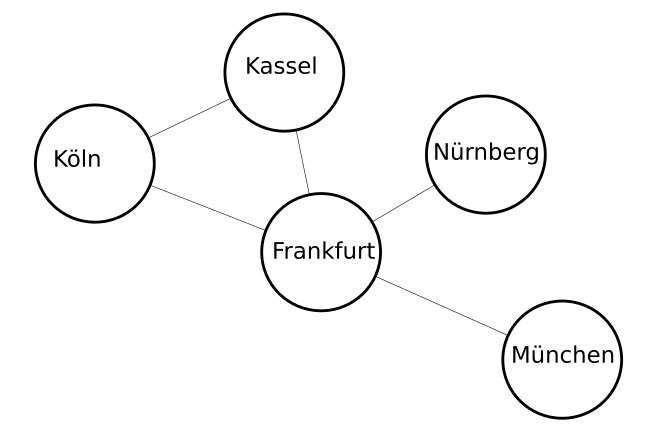
\includegraphics[scale=0.5]{bilder/einfachergraph}\label{fig_einfachergraph}
	}\\
	\caption[Einfacher Graph mit Städten als Knoten und deren Höchstspannungsleitungen als Kanten]{Einfacher Graph mit Städten als Knoten und deren Höchstspannungsleitungen als Kanten}
	\label{fig_einfachergraph}
\end{figure}


\begin{figure}[t]
	\centering
	\subfigure[Planarer Graph mit einer nicht planaren Zeichnung]
	{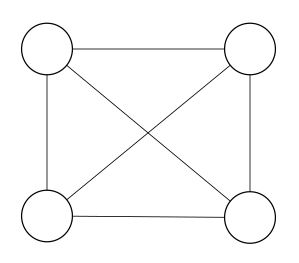
\includegraphics[scale=0.5]{bilder/planargraph1}\label{fig_planar1}
	}
	\hspace{1.0cm}%
	\subfigure[Planarer Graph mit einer planaren Zeichnung aber einer kurvigen Kante]
	{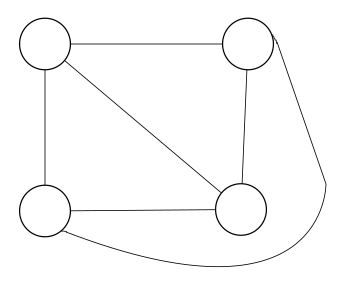
\includegraphics[scale=0.5]{bilder/planargraph3}\label{fig_planar2}
	}
	\hspace{1.0cm}%
	\subfigure[Planarer Graph mit planarer Zeichnung sowie geraden Kanten]
	{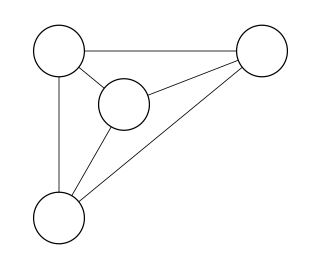
\includegraphics[scale=0.5]{bilder/planargraph2}\label{fig_planar3}
	}
	\\
	\caption[Verschiedene Zeichnungen eines planaren Graphen]{Verschiedene Zeichnungen eines planaren Graphen}
	\label{fig_testbild2}
\end{figure}
Ein Graph kann gerichtet oder ungerichtet sein. Bei einem ungerichteten Graphen gilt: $e_{v_{i},v_{j}} = e_{v_{j},v_{i}}$. Bei einem gerichteten Graphen gilt das nicht immer. Es wird der Kante somit eine Richtung mitgegeben. Ein Knoten $v_{i}$ hat eine Verbindung $e_{v_{i},v_{j}}$ zu einem anderen Knoten $v_{j}$, dies muss jedoch nicht bedeuten dass es auch eine Verbindung ausgehend von $v_{j}$ nach $v_{i}$ gibt. Es werden im Folgenden nur noch ungerichtete Graphen verwendet, somit gilt stets  $e_{v_{i},v_{j}} = e_{v_{j},v_{i}}$.\\

Gibt es keine Kante $e_{v_{i},v_{i}}$ mit $v_{i} \in V$ so ist der Graph schlingenfrei, es existiert also keine Kante von einem Knoten zu sich selbst. Eine Kante heißt demnach Schlinge sofern $e_{v_{i},v_{i}}$ gilt. \\

Kanten sind benachbart oder adjazent, sofern es zwei Knoten $v_{i},v_{j} \in V$ gibt und eine Kante $e_{v_{i},v_{j}} \in E$ sie verbindet. Da nur ungerichtete Graphen verwendet werden, ist es möglich den Start- sowie Endknoten einer Kante stets zu vertauschen und demnach ist auch $e_{v_{j},v_{i}} \in E$ adjazent. \\

Ein Pfad $w_{v_{n}, .., v_{m}}$ ist eine Folge von verbundenen Knoten ausgehend vom Knoten $v_{n}$ nach $v_{m}$ oder andersrum. Dabei sind die Knoten $v_{n}$ und $v_{m}$ Start- und Endknoten der Folge.    \\

Eines der wichtigsten Probleme in der Graphentheorie befasst sich mit dem Finden des kürzesten Pfades zweier Knoten in einem Graphen. Dieser kürzeste Pfad, auch Weg genannt, zwischen zwei unterschiedlichen Knoten $v_{i}$, $v_{j}$ ist der Pfad mit der minimalen Anzahl an Kanten vom Knoten $v_{i}$ nach $v_{j}$[Wikipedia]. \\

Bei einem Graph ist nicht nur die Einhaltung der eigentlichen Struktur wichtig sondern auch wie dessen Knoten und Kanten platziert werden, um eine übersichtliche und anschauliche Zeichnung zu erhalten. Eine wichtige Eigenschaft eines Graphen um dies zu erreichen ist die Planarität. Im Zweidimensionalen Raum ist ein Graph planar sofern es möglich ist diesen so zu zeichnen, dass sich keine Kanten überschneiden. Existiert eine solche Darstellung so ist es auch stets möglich den Graphen planar mit geraden Kanten zu zeichnen[2]. In Abbildung 2.7 ist der Unterschied zwischen dem planaren Graphen und seiner unterschiedlichen Zeichnungen zu sehen. Der planare Graph kann somit auch mit überschneidbaren Kanten gezeichnet werden, mit eckigen oder auch immer mit geraden Kanten. \\


Der Graph wird auf einer simplen Oberfläche im $R_{2}$ gezeichnet. Die Knoten werden jeweils durch ihre Koordinaten auf der Karte als Punkte dargestellt. Kanten sind an keinem expliziten Koordinatenpaar gebunden, werden jedoch indirekt durch die Koordinaten ihrer Knoten auf die Oberfläche gezeichnet. Existiert eine Kante $e_{v_{i},v_{j}} \in E$ so wird diese gezeichnet von der Position des Knotens $v_{i}$ zur Position des Knotens $v_{j}$. Durch das Koordinatenpaar der Knoten ist es demnach sehr einfach möglich den Graphen auf einer Oberfläche darzustellen. \\

Die Knoten werden als Punkte dargestellt, während die Kanten zwischen den Knoten als einfache gerade Striche gezeichnet werden. Es gibt jedoch viele weitere Methoden um dieses Struktur darzustellen. Die Knoten können ebenso mittels Boxen oder Vierecke dargestellt werden, Kanten als Kurven oder gestrichelte Linien[Algorithms for drawing graphs:an annotated bibliography *]. Die Größe und Farbe der einzelnen Knoten und Kanten können im Graph variieren und müssen nicht einheitlich gewählt werden. Dies ist sehr nützlich um bestimmte wichtige Knoten hervorzuheben oder um Beziehungen zwischen Knotengruppen darzustellen, indem ihnen alle die selbe Farbe zugewiesen wird oder ihnen die gleiche Form vergibt. Der Graph, der im Kapitel 2.3 erstellt wird hat zwei verschiedene Gruppen von Knoten. Die eine Knotengruppe lässt sich durch den Algorithmus im Kapitel drei verschieben, während die anderen Knoten zu den unbeweglichen Knoten gehören und ihre Position endgültig ist. Die unbeweglichen Knoten repräsentieren Große Städte und die beweglichen Knoten kleinere Städte und Abzweigungen. Um diese Knoten voneinander unterscheiden zu können sind die Knoten, die die größeren Städte repräsentieren, rot anstatt schwarz
 und wurden zur noch besseren Erkennbarkeit größer gezeichnet. Die Kanten wurden jedoch stets als schwarze Linien dargestellt, da es keine Unterschiede zwischen den Verbindungen in einem Höchstspannungsnetz gibt. 

\section{Vom Höchstspannungsnetz zum Graphen}
\label{Vom Höchstspannungsnetz zum Graphen}
%
\begin{figure}[t]
	\centering
	\subfigure[Ausschnitt des deutschen Höchstspannungsnetzes]
	{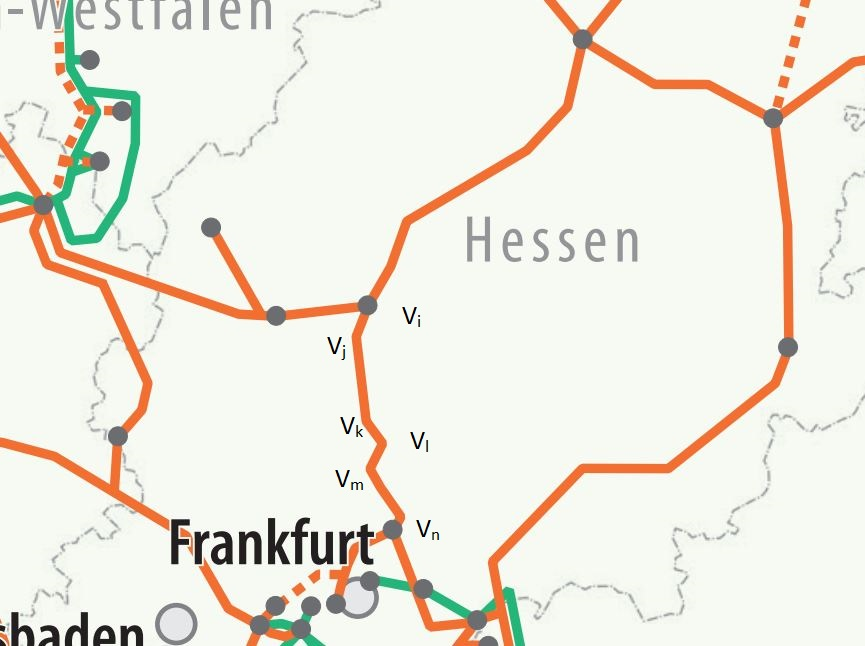
\includegraphics[scale=0.6]{bilder/Kartenausschnit2mitknoten}\label{fig_planar1}
	}
	\hspace{1.0cm}%
	\subfigure[Resultierender Graph aus der Karte]
	{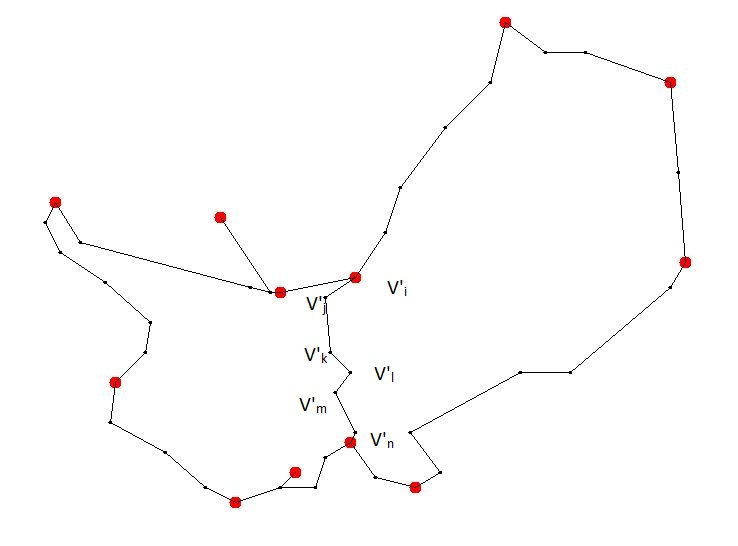
\includegraphics[scale=0.7]{bilder/ausschnittgraphmitknoten3}\label{fig_planar2}
	}
	\\
	\caption[Übergang von der Karte des Höchstspannungsnetzes zu einem Graphen]{Übergang von der Karte des Höchstspannungsnetzes zu einem Graphen}
	\label{fig_testbild2}
\end{figure}



In der Abbildung 2.x wird der Vorgang von einem Höchstspannungsnetz zu einem Graph dargestellt. In Abbildung 2.x(a) ist ein Ausschnitt des deutschen Höchstspannungsnetzes zu sehen. Gut zu erkennen sind die einzelnen Städte und ihre Verbindungen mittels den Höchstspannungsleitern. Diese Verbindungen repräsentieren einen Mast mit mehreren verschiedenen Leiterseilen. Die größeren Städte werden dabei als unbewegliche Knoten dargestellt. Ein Knoten ist unbeweglich, sofern er nicht mehr durch einen späteren Algorithmus verschoben werden kann, demnach ist seine Position endgültig. Die eigentlichen Positionen der Knoten werden mittels einfachen $x$ und $y$ Koordinaten zugewiesen. \\ 

\begin{figure}[t]
	\centering
	\subfigure[Resultierender Graph aus der Karte]
	{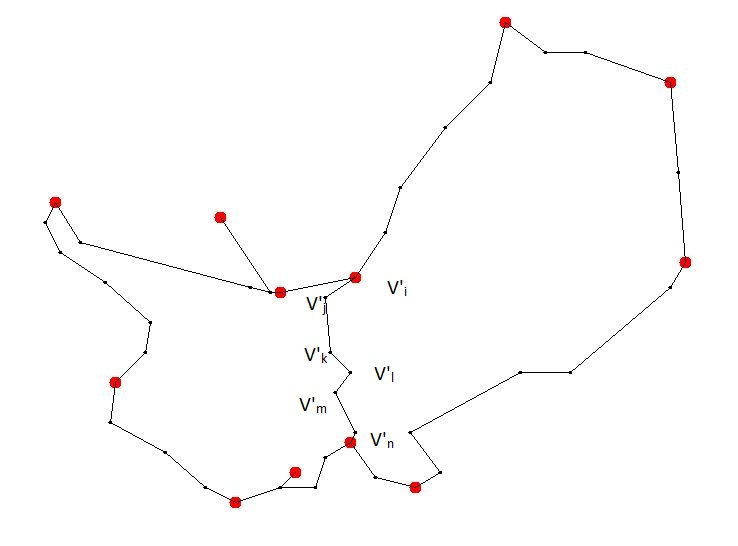
\includegraphics[scale=0.7]{bilder/ausschnittgraphmitknoten3}\label{fig_planar1}
	}
	\hspace{1.0cm}%
	\subfigure[Der Graph mit den modellierten Leiterseilen]
	{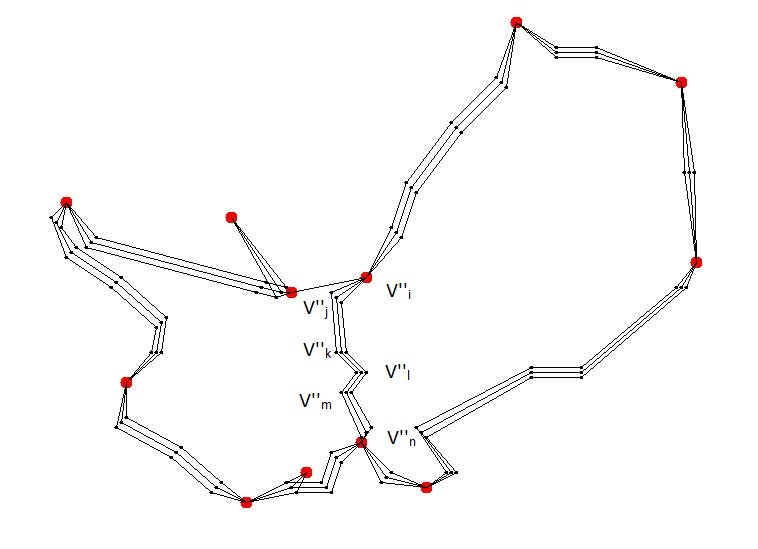
\includegraphics[scale=0.7]{bilder/ausschnittfertigergraph2}\label{fig_planar2}
	}
	\\
	\caption[Modellierung der Leiterseile]{Modellierung der Leiterseile}
	\label{fig_testbild2}
\end{figure}


Auf der Karte in der Abbildung 2.x(a) sind noch eckige Verbindungen zwischen den Städten zu sehen. Eine Verbindung auf dieser Karte repräsentiert den Verlauf der Leiterseile und die Positionen der Höchstspannungsmasten. Ist eine Ecke in der Verbindung zu sehen so wurden Hindernisse umgangen oder kleinere Orte vernetzt. Es ist nicht nötig jeden Mast auf der Karte auch als Knoten zu modellieren, da die späteren Kanten ohne Ecken verlaufen werden. Je mehr Masten als Knoten modelliert werden, desto besser werden die Verbindungen jedoch werden. Besonders wichtig sind die einzelnen Ecken der Verbindungen, diese müssen als Knoten modelliert werden, weil sonst der komplette Verlauf der Leiterseile im späteren Graphen verloren geht. Die Knoten $v_{i}^{'}$ und $v_{n}^{'}$ in der Abbildung 2.x(b) sind größere Städte und wurden dementsprechend zu unbewegliche Knoten. Die Knoten $v_{j}^{'}$ bis $v_{m}^{'}$ sind die Ecken im Verlauf der Verbindung der Karte in der Abbildung 2.x(a) und entsprechen ihren Masten $v_{j}^{'}$ bis $v_{m}^{'}$. Diese Knoten können durch spätere Verfahren verschoben werden. \\
\begin{figure}[t]
	\centering
	{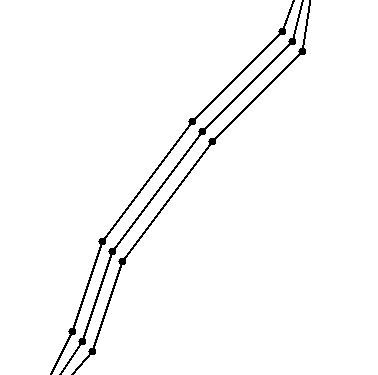
\includegraphics[scale=0.7]{bilder/knotenplacement}\label{fig_knotenplacement}
	}\\
	\caption[Erzeugung der neuen Knoten zur Modellierung der Leiterseile]{Erzeugung der neuen Knoten zur Modellierung der Leiterseile}
	\label{fig_knotenplacement}
\end{figure}

Um aus der Karte den abschließenden Graphen zu erhalten, der das Höchstspannungsnetz modelliert, müssen noch die einzelnen Leiterseile der Masten hinzugefügt werden. Bis jetzt wurden nur die Knoten und die grundlegenden Verbindungen modelliert. Auf der Karte in Abbildung 2.x(a) fehlen die Informationen um wie viele Leiterseile es sich bei den jeweiligen Verbindungen handelt. Das ist einer der grundlegenden Unterschiede zwischen einer normalen MetroMap und der neuen Darstellung die aus dem Höchstspannungsnetz resultiert. Bei einer MetroMap oder generell bei Bus- und Bahnverbindungen existieren nur sehr selten mehrere Straßen oder Gleise die immer mit der selben Verbindung verlaufen. Da dies jedoch der Fall ist bei einem Höchstspannungsnetz muss diese Eigenschaft extra modelliert werden. Im folgenden werden die Verbindungen immer mit genau drei Leiterseilen modelliert, anstatt die echten Werte zu nehmen, welche sich zwischen 1-5 Leiterseile befinden, das macht den Graphen für die spätere Handhabung überschaubarer. \\


Um die jeweiligen Leiterseile modellieren zu können wurden weitere bewegliche Knoten erstellt. Ein Knoten für jede Ecke einer Verbindung steht für das jeweilige Leiterseile an einem Mast. Diese Knoten wurden um den ursprünglichen Knoten platziert, sodass sich parallele Verlaufe gebildet haben, wie es auch bei einem echten Höchstspannungsnetz mit den Leiterseilen der Fall ist. Auf der Abbildung 2.x wird diese Verfahren dargestellt, der Knoten $v_{j}^{'}$ wird in Abbildung 2.x zu den drei Knoten $v_{i}^{''}$, $v_{j}^{''}$ und $v_{k}^{''}$, die jetzt den Mast mit den drei Leiterseilen repräsentieren. Da es drei Leiterseile pro Verbindung gibt, wurde die Anzahl der Kanten des resultierenden Graphen durch dieses Vorgehen fast verdreifacht.  





\section{MetroMap Layout Problem}
\label{MetroMap}
%
\begin{figure}[t]
	\centering
	{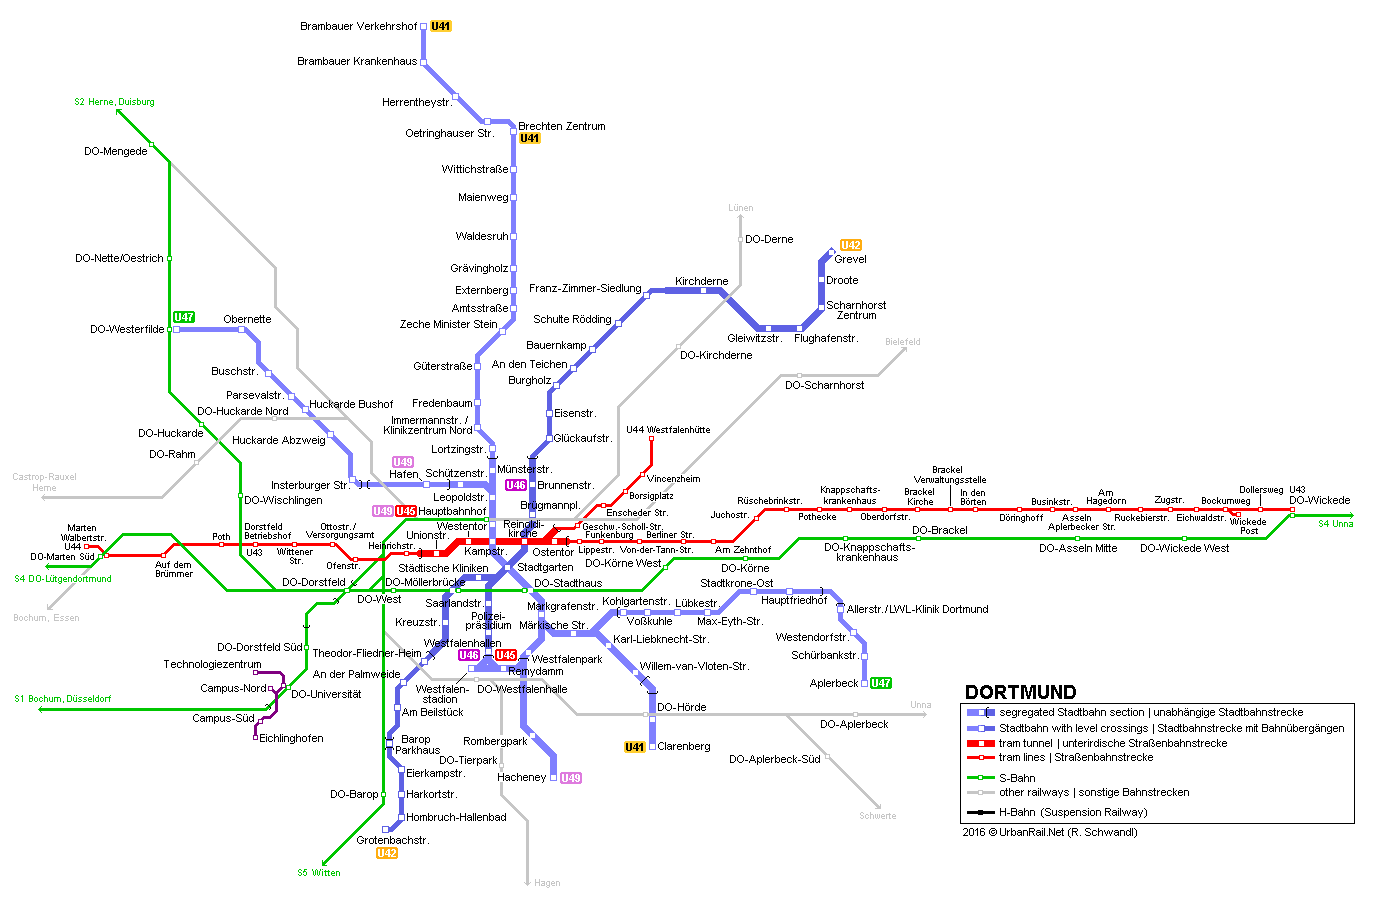
\includegraphics[scale=0.3]{bilder/dortmundmap}\label{fig_dortmundmap}
	}\\
	\caption[Dortmunder MetroMap]{Dortmunder MetroMap [http://www.urbanrail.net/eu/de/do/dortmund-map.png]}
	\label{fig_dortmundmap}
\end{figure}

Eine MetroMap ist die besondere Darstellungen eines Graphen, der aus einer Karte von verschiedensten Netzen gewonnen wird. Dieser Graph wird versucht so anschaulich wie möglich darzustellen, sodass es möglich ist die Struktur des Graphen schnellstmöglich zu verstehen und Verbindungen zwischen Knoten nachvollzogen werden können. Häufig werden allgemeine Netze wie das Bus- und Bahnnetz mittels einer MetroMap dargestellt, damit sind sie Bestandteil des täglichen Lebens. Viele benutzen sie zur schnellen Orientierung und Übersicht. Eine MetroMap macht aus, dass sie schnell zu lesen und zu verstehen ist. Es muss demnach möglich sein die benötigen Informationen in kurzer Zeit und sicher aus der Karte zu erhalten. \\

MetroMaps dienen hauptsächlich dazu die richtige Bahn oder Bus zum gewünschten Ziel zu nehmen und sich eine gute Übersicht der Lage zu verschaffen. Die geographisch echten Karten mit ihren Verzweigungen und Überschneidungen erfüllen diesen Zweck nicht. In Abbildung 2.9 wird eine Dortmunder MetroMap der lokalen Bahnverbindungen gezeigt. Fast alle vorhandenen MetroMaps von Bahn- und Busnetzwerken wurden per Hand gezeichnet, jedoch ist es auch möglich dies mittels Algorithmen zu tun. Es gibt bereits viele verschiedene Algorithmen sowie Ansätze die MetroMaps automatisch aus einem Graphen generieren. Um diese zu behandeln muss zu erst geklärt werden was genau eine MetroMap ist und was diese ausmacht. \\

Eine essentielle Eigenschaft die der Graph der MetroMap haben sollte ist die Planarität. Wird der Graph wie ein Labyrinth gezeichnet mit überlappenden Kanten, so wird diese fast unmöglich für den alltäglichen Gebrauch zu benutzen sein.

\begin{figure}[t]
	\centering
	{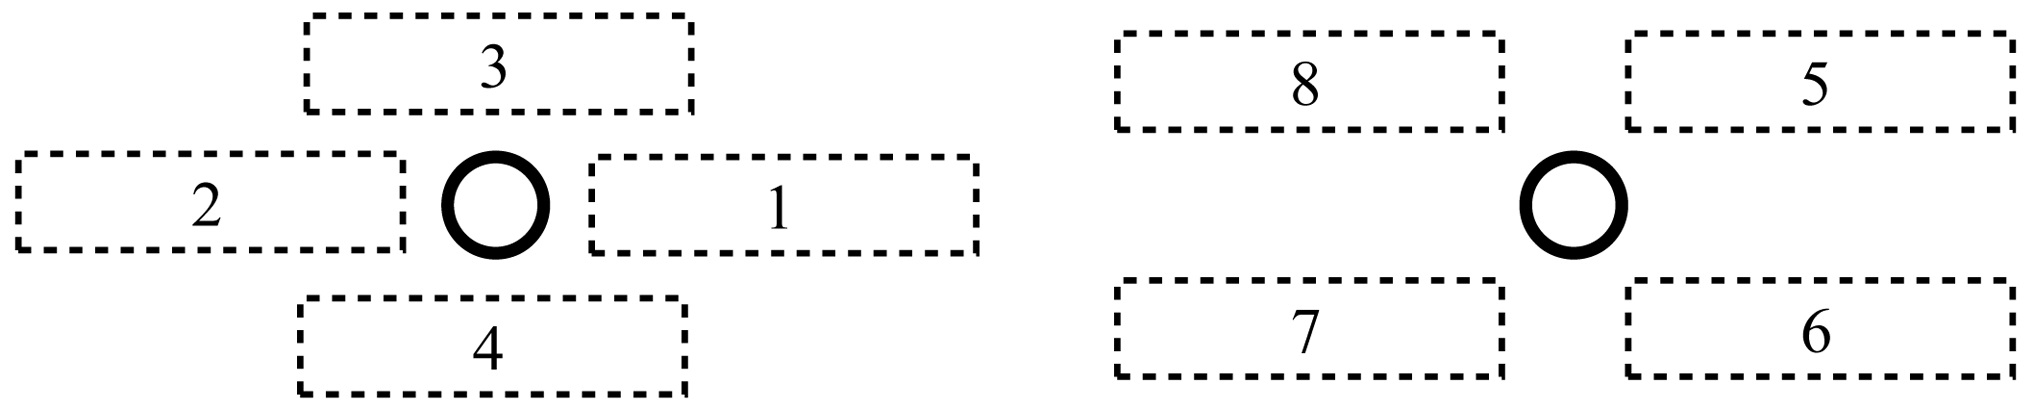
\includegraphics[scale=0.25]{bilder/labelplacements}\label{fig_labelplacements}
	}\\
	\caption[8 Mögliche Platzierungen der Beschriftung]{8 Mögliche Platzierungen der Beschriftung [http://doi.ieeecomputersociety.org/cms/Computer.org/dl/ trans/tg/2011/01/figures/ttg20110101018.jpg]}
	\label{fig_labelplacements}
\end{figure}

Eine weitere Sache die entscheidend dazu beiträgt die resultierende Karte möglichst übersichtlich zu gestalten ist die Vermeidung von eckigen und runden Kanten. Es ist viel einfacher den gewollten Weg auf einer senkrechten bzw. waagerechten Strecke zu verfolgen als wenn dieses über eckige und runde Kanten geschieht. \\

Bei einer MetroMap ist es sehr wichtig zu unterscheiden um welche Art der Verbindung es sich handelt. Denn ein Bus fährt nicht auf Gleisen und Züge nicht auf Straßen, somit müssen unterschiedliche Verbindungen gekennzeichnet werden. Dafür werden die jeweiligen Pfade $w_{v_{n}, .., v_{m}}$ im Graphen aufgestellt, die diese Verbindungen repräsentieren. Hierbei sind die Knoten $v_{n}$ und $v_{m}$ jeweils die letzten Stationen der Verbindung. Diese können nun auf unterschiedliche Weise gekennzeichnet werden, durch Färbung, Umrandung oder indem die Verbindung verschieden gestrichelt wird. \\

Eine MetroMap verliert ihre Eigenschaft der Topologie sowie der geographischen Richtigkeit im Vergleich zu einer normalen Karte, dies resultiert zwingend aus der Verschiebung der Knoten und Kanten um einen übersichtlicheren Graphen zu bekommen. Da die Verbindungen aus den realen Netzen modelliert wurden, wird stets eine gewisse Topologie beibehalten beim Erstellen der MetroMap. Dabei wird der geographische Abstand zwischen zwei Punkten vernachlässigt. Die Lage der ursprünglichen Stationen ist zur Bewahrung der Navigation da weitaus wichtiger. Es würde auch stark verwirren wenn eine Verbindung von A über B nach C geht, die eigentlichen Stationen auf der Karte jedoch in Reihenfolge A C B gezeichnet werden. Dies würde auch im Widerspruch dazustehen, gerade Kanten aufrechtzuerhalten und ganze Verbindungen möglichst senkrecht und waagerecht zu zeichnen. \\

Neben der Platzierung der Kanten und Knoten ist es sehr wichtig eine passende Beschriftung der Objekte in der MetroMap zu haben. Für diese Beschriftungen muss es den Platz geben, da sich die Beschriftungen nicht mit den Kanten oder Knoten überschneiden dürfen. Wenn der Abstand zwischen den jeweiligen Beschriftungen der Kanten und Knoten zu weit oder zu nah ist, wird es schwierig zu erkennen zu welchem Objekt diese gehört. \\

Ein möglicher Ansatz dieses Problem zu lösen wäre es jedem Objekt eine gewisse Anzahl von möglichen Beschriftungspositionen zu geben und anschließend die sich überschneidenden Positionen als mögliche Beschriftungen zu streichen. Was bleibt sind überschneidungsfreie Beschriftungen eines jeden Objektes. Es müssen demnach zu erst die möglichen Beschriftungspositionen eines Objektes gefunden werden. Dazu werden 8 Positionen um das jeweilige Objekt gewählt, wie in der Abbildung 2.x dargestellt. Es ist nun möglich diesen Positionen eine Wertigkeit zuzuweisen. Im $45$ Winkel zum Objekt, wäre die Beschriftung generell am besten platziert um einen übersichtlichen Graphen zu bekommen. Nun ist es leicht die beste überschneidungsfreie Beschriftung mit den geringsten Kosten zu finden. Die Kosten stellen die Wertigkeit der Positionen aller Beschriftungen der Objekte.  